\documentclass[air,article,submit,moreauthors]{Definitions/mdpi}

% Supplementary materials: S-prefixed table and figure numbering.
\renewcommand{\thetable}{S\arabic{table}}
\renewcommand{\thefigure}{S\arabic{figure}}
\usepackage{tabularx}

\firstpage{1}
\makeatletter
\setcounter{page}{\@firstpage}
\makeatother
\pubvolume{1}
\issuenum{1}
\articlenumber{0}
\pubyear{2026}
\copyrightyear{2026}
\datereceived{ }
\daterevised{ }
\dateaccepted{ }
\datepublished{ }

\Title{Supplementary Materials: WRF Cold-Pool Sensitivities Relevant to Winter-Ozone Modelling in the Uinta Basin}

\newcommand{\orcidauthorA}{0000-0003-0305-4090}
\newcommand{\orcidauthorB}{0009-0009-9083-6568}
\Author{John R. Lawson $^{1,2,}$*\orcidA{}, Michael J. Davies $^{1}$\orcidB{}, Loknath Dhar $^{1,3}$ and Seth N. Lyman $^{1,3}$}
\AuthorNames{John R. Lawson, Michael J. Davies, Loknath Dhar and Seth N. Lyman}

\address{%
$^{1}$ \quad Bingham Research Center, Utah State University, Vernal, UT 84078, USA;\\
$^{2}$ \quad Department of Mathematics and Statistics, Utah State University, Logan, UT 84322, USA;\\
$^{3}$ \quad Department of Chemistry and Biochemistry, Utah State University, Logan, UT 84322, USA}
\corres{Correspondence: john.lawson@usu.edu}

\abstract{This document collects bounded secondary diagnostics that support the main article.
It does not change the controlled driving-product result or the status of any predeclared gate.}

\begin{document}

These supplementary materials retain bounded secondary diagnostics from the 2 February 2013 Uinta Basin WRF case.
They do not change the article's controlled driving-product result or the status of its failed gates.

\begin{table}[H]
\caption{Controlled process-treatment effects on the frozen station/common-AGL pipeline.
Values are means of five hourly spatial medians; signs are positive/negative hours with exact zeros omitted.
Planetary boundary-layer height is scheme defined across the boundary-layer/surface-layer treatment.}
\label{tab:s1-process-effects}
\centering
\footnotesize
\begin{tabular}{lrrrr}
\toprule
Metric & \multicolumn{2}{c}{Slope radiation (X1 $-$ X0)} & \multicolumn{2}{c}{MYJ/Eta (X2 $-$ X1)} \\
 & Mean & Signs & Mean & Signs \\
\midrule
T2 bias ($^{\circ}$C) & +0.001 & 3/1 & +0.37 & 5/0 \\
10 m wind absolute error (m s$^{-1}$) & +0.001 & 2/2 & -0.145 & 0/5 \\
Surface-pressure bias (Pa) & -0.12 & 0/4 & +6.3 & 5/0 \\
Stability $S_{50:500}$ (K) & +0.004 & 3/1 & +0.11 & 3/2 \\
Transport wind $U_{50:500}$ (m s$^{-1}$) & +0.006 & 4/0 & +0.098 & 5/0 \\
PBL height (m) & +0.01 & 3/1 & -9.2 & 2/3 \\
\bottomrule
\end{tabular}
\end{table}

\begin{table}[H]
\caption{Static-terrain diagnostics retained after the failed default-minus-fine gate and the closed coarse-member lineage check.}
\label{tab:s2-terrain-summary}
\centering
\small
\begin{tabularx}{\textwidth}{lXXX}
\toprule
Contrast & Terrain difference & 2 m response & Status \\
\midrule
Default minus fine & 7.9 m RMS; -55 to +60 m range & Elevation-band means 0.07--0.27 K; terrain correlation below 0.3 at 1400--1600 UTC & Predeclared conjunction failed \\
Coarse brackets & 91.9/93.1 m RMS; extrema to -462/+487 m & Slope-band means 1.2--1.5 K; terrain correlation 0.50--0.67 & Descriptive only; no predeclared gate \\
Coarse-member lineage & As-run namelist matches the controlled family; terrain is materially smoother & Configuration caveat closed & Supports controlled-bracket status, not a terrain ranking \\
\bottomrule
\end{tabularx}
\end{table}

\begin{figure}[H]
\centering
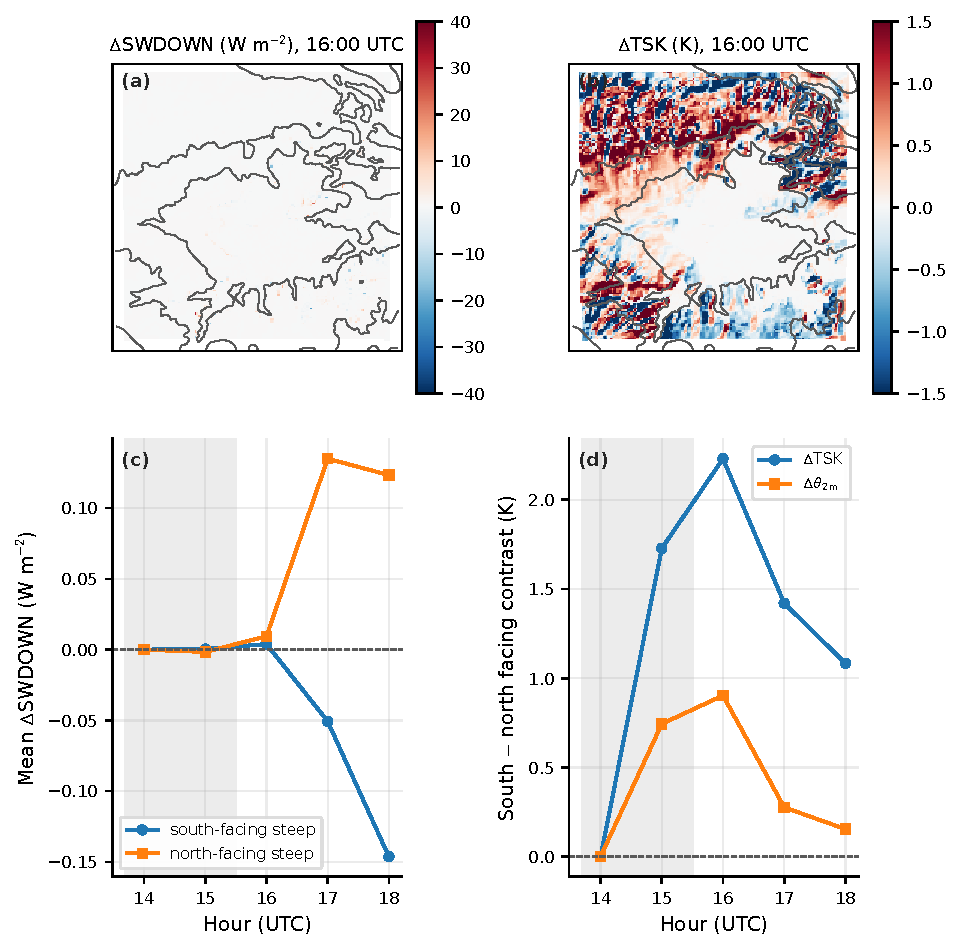
\includegraphics[width=0.92\textwidth]{figures/wrf_radiation_response_cmp07_d02.pdf}
\caption{Diagnostic for the slope-radiation screen, calculated as X1 minus X0 on d02.
The archived flat-plane shortwave field did not express the treatment, while skin temperature showed an aspect-organised response on steep terrain.
The predeclared screen failed for this measurement-limited reason, and the figure does not support a configuration ranking or a claim that slope-aware radiation improved or degraded the cold pool.}
\label{fig:s1-radiation-response}
\end{figure}

\end{document}
